\documentclass[10pt,landscape,a4paper]{article}
\PassOptionsToPackage{usenames,dvipsnames}{xcolor}
\usepackage[utf8]{inputenc}
\usepackage[UKenglish]{babel}
\usepackage{tikz}
\usetikzlibrary{shapes,positioning,arrows,fit,calc,graphs,graphs.standard}
\usepackage[nosf]{kpfonts}
\usepackage[t1]{sourcesanspro}
\usepackage{multicol}
\usepackage{wrapfig}
\usepackage[top=0mm,bottom=4mm,left=2mm,right=1mm]{geometry}
\usepackage[framemethod=tikz]{mdframed}
\usepackage{microtype}
\usepackage{mathtools} % loads amsmath, for math environments etc
\usepackage{setspace}
\usepackage{tikz}
\usetikzlibrary{trees}
\usepackage{enumitem}
\usepackage{kpfonts,amssymb,empheq,fancybox}
\usepackage{mathtools}
\usepackage{venndiagram}
\usepackage{enumitem}
\usepackage{pgfplots}
\usepackage{textcomp}
\usepackage{scalerel}
\usepackage{wasysym}
\usepackage{pagecolor}

%%highliht with \hl
\usepackage{xcolor}
\usepackage{soul}
\colorlet{highlightgreen}{green!10}
\sethlcolor{highlightgreen}




\DeclareRobustCommand{\hly}[1]{{ 
		\colorlet{highlightyellow}{Salmon!30}
		\sethlcolor{highlightyellow} 
		\hl{#1}}}

\DeclareRobustCommand{\hlr}[1]{{ 
		\colorlet{highlight}{red!60}
		\sethlcolor{highlight} 
		\hl{#1}}}

\setitemize{leftmargin=*,noitemsep,topsep=0pt,parsep=0pt,partopsep=0pt}

\let\bar\overline
\let\displaystyle\textstyle

\definecolor{myblue}{cmyk}{1,.72,0,.38}

\def\firstcircle{(0,0) circle (1.5cm)}
\def\secondcircle{(0:2cm) circle (1.5cm)}

\colorlet{circle edge}{myblue}
\colorlet{circle area}{myblue!5}

\tikzset{filled/.style={fill=circle area, draw=circle edge, thick},
    outline/.style={draw=circle edge, thick}}

\pgfdeclarelayer{background}
\pgfsetlayers{background,main}

\everymath\expandafter{\the\everymath \color{myblue}}
\everydisplay\expandafter{\the\everydisplay \color{myblue}}

\renewcommand{\baselinestretch}{.8}
\pagestyle{empty}

\global\mdfdefinestyle{header}{%
linecolor=gray,linewidth=1pt,%
leftmargin=6mm,rightmargin=6mm,skipbelow=1mm,skipabove=1mm,
}

\newcommand{\ffbox}[1]{%
	{% open a group for a local setting
		\setlength{\fboxsep}{-2\fboxrule}% the rule will be inside the box boundary
		\fbox{\hspace{1.2pt}\strut#1\hspace{1.2pt}}% print the box, with some padding at the left and right
	}% close the group
}

\newcommand{\header}{
\begin{mdframed}[style=header]
\scriptsize

\textbf{Stefanica - 150 quant interviews \\ ~Alain~Chenier,~page~\thepage,  \today{} }
\end{mdframed}
}

\makeatletter
\renewcommand{\section}{\@startsection{section}{1}{0mm}%
                                {.1ex}%
                                {.1ex}%x
                                {\color{blue}\sffamily\small\bfseries}}
\renewcommand{\subsection}{\@startsection{subsection}{1}{0mm}%
                                {.1ex}%
                                {.1ex}%x
                                {\sffamily\bfseries}}

\def\textSq#1{%
	\begingroup% make boxes and lengths local
	\setlength{\fboxsep}{0.001pt}% SET ANY DESIRED PADDING HERE
	\setbox1=\hbox{#1}% save the contents
	\setlength{\@tempdima}{\maxof{\wd1}{\ht1+\dp1}}% size of the box
	\setlength{\@tempdimb}{(\@tempdima-\ht1+\dp1)/2}% vertical raise
	\raise-\@tempdimb\hbox{\fbox{\vbox to \@tempdima{%
				\vfil\hbox to \@tempdima{\hfil\copy1\hfil}\vfil}}}%
	\endgroup%
}
\def\Sq#1{\textSq{\ensuremath{#1}}}%

\def\multi@column@out{%
   \ifnum\outputpenalty <-\@M
   \speci@ls \else
   \ifvoid\colbreak@box\else
     \mult@info\@ne{Re-adding forced
               break(s) for splitting}%
     \setbox\@cclv\vbox{%
        \unvbox\colbreak@box
        \penalty-\@Mv\unvbox\@cclv}%
   \fi
   \splittopskip\topskip
   \splitmaxdepth\maxdepth
   \dimen@\@colroom
   \divide\skip\footins\col@number
   \ifvoid\footins \else
      \leave@mult@footins
   \fi
   \let\ifshr@kingsaved\ifshr@king
   \ifvbox \@kludgeins
     \advance \dimen@ -\ht\@kludgeins
     \ifdim \wd\@kludgeins>\z@
        \shr@nkingtrue
     \fi
   \fi
   \process@cols\mult@gfirstbox{%
%%%%% START CHANGE
\ifnum\count@=\numexpr\mult@rightbox+2\relax
          \setbox\count@\vsplit\@cclv to \dimexpr \dimen@-1cm\relax
\setbox\count@\vbox to \dimen@{\vbox to 1cm{\header}\unvbox\count@\vss}%
\else
      \setbox\count@\vsplit\@cclv to \dimen@
\fi
%%%%% END CHANGE
            \set@keptmarks
            \setbox\count@
                 \vbox to\dimen@
                  {\unvbox\count@
                   \remove@discardable@items
                   \ifshr@nking\vfill\fi}%
           }%
   \setbox\mult@rightbox
       \vsplit\@cclv to\dimen@
   \set@keptmarks
   \setbox\mult@rightbox\vbox to\dimen@
          {\unvbox\mult@rightbox
           \remove@discardable@items
           \ifshr@nking\vfill\fi}%
   \let\ifshr@king\ifshr@kingsaved
   \ifvoid\@cclv \else
       \unvbox\@cclv
       \ifnum\outputpenalty=\@M
       \else
          \penalty\outputpenalty
       \fi
       \ifvoid\footins\else
         \PackageWarning{multicol}%
          {I moved some lines to
           the next page.\MessageBreak
           Footnotes on page
           \thepage\space might be wrong}%
       \fi
       \ifnum \c@tracingmulticols>\thr@@
                    \hrule\allowbreak \fi
   \fi
   \ifx\@empty\kept@firstmark
      \let\firstmark\kept@topmark
      \let\botmark\kept@topmark
   \else
      \let\firstmark\kept@firstmark
      \let\botmark\kept@botmark
   \fi
   \let\topmark\kept@topmark
   \mult@info\tw@
        {Use kept top mark:\MessageBreak
          \meaning\kept@topmark
         \MessageBreak
         Use kept first mark:\MessageBreak
          \meaning\kept@firstmark
        \MessageBreak
         Use kept bot mark:\MessageBreak
          \meaning\kept@botmark
        \MessageBreak
         Produce first mark:\MessageBreak
          \meaning\firstmark
        \MessageBreak
        Produce bot mark:\MessageBreak
          \meaning\botmark
         \@gobbletwo}%
   \setbox\@cclv\vbox{\unvbox\partial@page
                      \page@sofar}%
   \@makecol\@outputpage
     \global\let\kept@topmark\botmark
     \global\let\kept@firstmark\@empty
     \global\let\kept@botmark\@empty
     \mult@info\tw@
        {(Re)Init top mark:\MessageBreak
         \meaning\kept@topmark
         \@gobbletwo}%
   \global\@colroom\@colht
   \global \@mparbottom \z@
   \process@deferreds
   \@whilesw\if@fcolmade\fi{\@outputpage
      \global\@colroom\@colht
      \process@deferreds}%
   \mult@info\@ne
     {Colroom:\MessageBreak
      \the\@colht\space
              after float space removed
              = \the\@colroom \@gobble}%
    \set@mult@vsize \global
  \fi}

\makeatother

\newcommand{\myE}[1]{ \mathbb{E} \left[ #1 \right] }
\newcommand{\mycondE}[2]{E \left( #1 | #2 \right) }
\newcommand{\myMI}{ M_{\infty} }
\newcommand{\myMn}{ M_{n} }
\newcommand{\myM}[1]{M_{#1}}

\newcommand{\myFF}{\mathcal{F}}
\newcommand{\myGF}{\mathcal{G}}

\newcommand\myeq[1]{\stackrel{{\normalfont\mbox{#1}}}{ = }}
\newcommand\myle[1]{\stackrel{{\normalfont\mbox{#1}}}{ \le }}

\newcommand\myright[1]{\stackrel{{\normalfont\mbox{#1}}}{ \Rightarrow }}

\newcommand{\myVar}{ \operatorname{Var} }
\newcommand{\Var}{ \operatorname{Var} }

\def\stretchint#1{\vcenter{\hbox{\stretchto[440]{\displaystyle\int}{#1}}}}
\def\scaleint#1{\vcenter{\hbox{\scaleto[3ex]{\displaystyle\int}{#1}}}}

\newcommand\myexp[1]{e^{#1}}

\newcommand{\mylp}{ \left ( }
\newcommand{\myrp}{ \right ) }

\newcommand{\myblp}{ \big \{ }
\newcommand{\mybrp}{ \big \} }

\setlength{\parindent}{0pt}
\setlength{\columnseprule}{0.01pt}

\newcommand{\Tau}{\mathcal{T}}
\newcommand{\myhighlight}[1]{\colorbox{green!10}{$\displaystyle #1$}}

\def\bs{\mkern-7mu} % reset amount of backspacing for lower limit of integration

\newcommand{\myint}{\scaleint{4ex}}
\newcommand{\mybint}{\scaleint{7ex}}
\newcommand{\mybbint}{\scaleint{9ex}}
\newcommand{\sech}{ \operatorname{sech} }
\newcommand{\rpm}{\raisebox{.2ex}{$\scriptstyle\pm$}}

\newcommand*\dif{\mathop{}\!\mathrm{d}}

\definecolor{light-gray}{gray}{0.97}



\begin{document}

\newcommand{\sucht}{\ \wasytherefore\ }

\pagecolor{light-gray}	
\normalsize

\begin{multicols*}{4}

\begin{spacing}{0.1}
	
\section{2 put options , K=20,30 trading for \$4,\$6 - find arbitrage}
\begin{itemize}
	\item 2x6-3x4=0, so try  $2{(20-S)}^+ - 3{(30-S)}^+ > 0 $
	\item 
	$
	\begin{cases}
		S \ge 30 \Rightarrow 0 \\ 
		20 \le S \le 30 \Rightarrow \text{-ve} \\
		0 \le S \le 20 \Rightarrow \text{-ve}
	\end{cases}
	$
	\item 0 or -ve, so take opposite and done	
	\item graph (K,P(K)) not \textbf{strictly} convex $\Rightarrow$ arbitrage
	
	
\end{itemize}

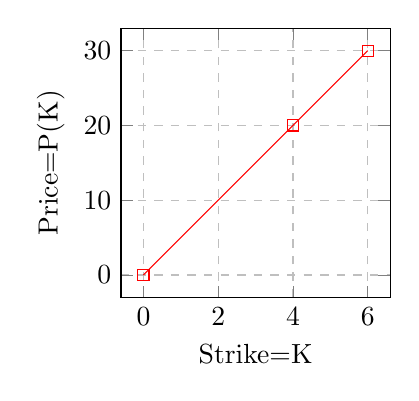
\begin{tikzpicture}
\begin{axis}[xlabel={Strike=K},ylabel={Price=P(K)},height=5cm,width=5cm,
ymajorgrids=true,xmajorgrids=true,grid style=dashed]
\addplot[color=red,mark=square] coordinates {(0,0)(4,20)(6,30)};
\end{axis}
\end{tikzpicture}


\section{$2^{29}$ has 9 digits all different - find missing digit}
\begin{itemize}
\item key: 9 divides [n - Sum(digits n)]
\item \textbf{Proof}: $n=a_n 10^n + a_{n-1} 10^{n-1}+ \ldots + a_{1} 10^{1} + a_0 $
\item $S(n)=a_n + a_{n-1}+ \ldots + a_{1} + a_0 $
\item $n-S(n)=a_n (10^n-1) + a_{n-1} (10^{n-1}-1)+ \ldots + a_{1} (10^1-1) + a_0-a_0 $
\item $10^k-1$ = all 9s = divisible by 9. so  QED
\item Sum(digits n) = $\sum_{1}^{9}i-x=45-x$
\item so $9|(2^{29}-45-x)$ 
\item but $2^{29}=2^5 \times 2^{6 \times 4} = 2^5 \times {64}^4= 2^5 \times {(63+1)}^4=2^5 \times {(k \times 63)+1}=k \times 63 \times 2^5+2^5 = 9 \times$ something for some k
\item so $9|(2^{29}-45-x)$ and $9|(2^{29}-2^5)$ so $9|(2^{29}-45-x)-(2^{29}-2^5)$
\item $9|(45-x-2^5)=(45-x-32)=(13-x)$ so $x=4$
\end{itemize}

\section{$\int_0^T W_t dt$ - what is distribution ? is it martingale ?}
\begin{itemize}
\item $X_T=\int_0^T W_t dt \Leftrightarrow dX_t=W_tdt+0.dW_t$ =  only drift so not martingale
\item $dX_t=W_tdt \Leftrightarrow X_T=\int_0^T W_t dt \Leftrightarrow X_T = [W_tt]_0^T - \int_{0}^{T}tdW_t = TW_T- \int_{0}^{T}tdW_t = T\int_{0}^{T}dW_t - \int_{0}^{T}tdW_t  = \int_{0}^{T} (T-t) dW_t$
\item Recall stochastic integral \colorbox{green!10}{ $\int_0^T f(t)dW_t \sim N(0,\int_{0}^{T}{|f(t)|}^2 dt)$}
\item $X_T=\int_{0}^{T} (T-t) dW_t \sim N(0,\int_0^T {|T-t|}^2)dt=N(0,{T^3 \over 3})$
\end{itemize}
\section{Alice sends 20 ants towards Bob in straight line, Bob 50 towards Alice in straight line. Ants collide and go back. How many reach Bob? Alice ? How many collisions ?}
\begin{itemize}
\item imagine ants carry a flag and pass it on. so 50 reach Alice and 20 reach Bob.
\item num collisions: each of Bob's 50 flags must go though 20 collisions to reach Alice, each of Alice's 20 flags goes through 50 collisions to reach Bob: 2x 50 x 20 = 2000 collisions
\end{itemize}

\section {find all $p$ such that this is a collrelation matrix} $\Omega = \begin{bmatrix} 1 & 0.6 & -0.3 \\  0.6 & 1 & p \\  -0.3 & p & 1 \end{bmatrix}$
\begin{itemize}
\item $\Omega$ correlation matrix $ \Leftrightarrow \Omega$ symmetric positive definite
\item \textbf{Sylvester}, \textbf{Cholesky} , \textbf{definition}
\item \textbf{Sylvester} criterion: all the principal minor determinants must be >0 (principal minor: remove the same rows  and same column indices form a matrix)
\begin{enumerate}
\item remove 2,3 $ \rightarrow \det (1) =1$, remove 1,3 $ \rightarrow  \det (1) =1$,  remove 1,2 $ \rightarrow  \det (1) =1$
\item remove 3 $\rightarrow \det \begin{bmatrix} 1 & 0.6 \\  0.6 & 1 \end{bmatrix} = 0.64$
\item remove 2 $\rightarrow \det \begin{bmatrix} 1 & -0.3 \\  -0.3 & 1 \end{bmatrix}=0.91$
\item remove 1 $\rightarrow \det \begin{bmatrix} 1 & p \\  p & 1 \end{bmatrix} = 1 -p^2$
\item remove $\emptyset \rightarrow \det \Omega =  \det \begin{bmatrix} 1 & 0.6 & -0.3 \\  0.6 & 1 & p \\  -0.3 & p & 1 \end{bmatrix}  \rightarrow \begin{bmatrix} 1 & 0.6 & -0.3  & 1 & 0.6 \\  0.6 & 1 & p & 0.6 & 1 \\  -0.3 & p & 1 & -0.3 & p \end{bmatrix} \rightarrow $ + down - up  $ \rightarrow 1 -0.18p -0.18p - 0.09 -p^2 -0.36 = 0.55 -0.36p -p^2$
\end{enumerate}
\item $\begin{cases} 1-p^2 > 0 \\ 0.55 -0.36p -p^2 >0 \end{cases}$
\end{itemize}

\section {how many draws N of U[0,1] such that $P(0.7 < U[0,1] < 0.72) \ge 0.95$ for one $U[0,1]$}
\begin{itemize}
\item P(none of the N rv in $[0.7,0.72]$)=${0.98}^N \rightarrow $ P(at least one in [0.7,0.72]) = $1-{0.98}^N$ and solve $1-{0.98}^N \ge 0.95$
\end{itemize}

\section {prove pdf of N(0,1) is $: \int \text{pdf}=1$}
\begin{itemize}
\item $\frac{1}{\sqrt{2\pi}} \int_{-\infty}^{+\infty} \exp(-{x^2 \over 2}) dx$ substitute $x^2/2 = t \rightarrow dx = \sqrt{(2)}dt \rightarrow $ need prove $ I := \int_{-\infty}^{+\infty} \exp(-{t^2}) dt = \sqrt{\pi } $

\item $I^2=\int_{-\infty}^{+\infty} \exp(-{x^2}) dx \int_{-\infty}^{+\infty} \exp(-{y^2}) dy = \int_{-\infty}^{+\infty} \exp(-{x^2+y^2}) dx dy $
\item $x=r\cos \theta , y = r \sin \theta , dxdy = rdrd\theta$
\item $I^2=\int_{0}^{+\infty}\int_{0}^{+2\pi} \exp(-r^2)rdrd\theta = 2\pi\int_{0}^{+\infty} \exp(-r^2)rdr = 2\pi {[{-1 \over 2}\exp(-r^2)]}_0^{+\infty}=\pi \rightarrow I= \sqrt{\pi} $
\end{itemize}

\section {walk 1m south, 1m east, 1m north, then back at same point - where are you o Earth?}
\begin{itemize}
\item find latitute near south Pole such that round-the-world=1m. then any point 1m north of this works
\item also any latitude near south Pole such that round-the-world=$1\over k$ works (go round the world k times but still end up same point)
\end{itemize}

\section {solve Oernstein-Uhlenbeck SDE - Vasicek for IR}
\begin{itemize}
\item $dr_t=\lambda(\theta-r_t)dt + \sigma dW_t \rightarrow dr + \lambda r_t dt=\lambda \theta dt + \sigma dW_t \myright {$\times e^{\lambda t}$} e^{\lambda t}(dr + \lambda r_t dt)=e^{\lambda t} (\lambda \theta dt + \sigma dW_t) \rightarrow d(r_t e^{\lambda t} ) = e^{\lambda t} (\lambda \theta dt + \sigma dW_t) \rightarrow {[r_t e^{\lambda t}]}_0^t = \int_{0}^t \lambda \theta e^{\lambda s} ds + \int_{0}^t \sigma e^{\lambda s}dW_s \rightarrow r_t e^{\lambda t}-r_0 = \theta (e^{\lambda t}-1) + \sigma \int_{0}^t  e^{\lambda s}dW_s \rightarrow r_t = e^{-\lambda t}r_0 + \theta (1-e^{-\lambda t}) + \sigma \int_{0}^t e^{-\lambda(s-t)} dW_s$ and that is it.
\item note however $E( \int_{0}^t f(s)dW_s)$ = "sum of N(0,.)"=0 so $E(r_t)= e^{-\lambda t}r_0 + \theta (1-e^{-\lambda t}) $ which $\rightarrow \theta$ as $r \uparrow +\infty$ "mean reverting"
\end{itemize}
\hrule

\section {Calculus}
\begin{itemize}
\item $\myhighlight{i^i ?}$ $e^{i\frac{\pi}{2}i}=e^{-\frac{\pi}{2}}$

\item $\myhighlight{\pi^e >< e^\pi ?}$ try $\ln(\pi^e)=e\ln(\pi)$ vs $ln(e^\pi)=\pi\ln(e)$ ie $\frac{\ln(\pi)}{\pi}$ vs $\frac{\ln(e)}{e}$ ie check $f(x)=\frac{\ln(x)}{x}$ ie $f'(x)=(\frac{\ln(x)}{x})'=\frac{1}{x}\frac{1}{x}+\ln(x)\frac{-1}{x^2}=\frac{1-\ln x}{x^2}$ ie $f'(x)<0$ if $x >e$ and $f'(x)>0$ if $x <e$ ie $f(x) \uparrow$ on $[0,e]$ and $f \downarrow$ on $[e,...+\infty]$ and $e<\pi$ so $f(e)>f(\pi)$

\item $\myhighlight{ \frac{e^x+e^y}{2} > e^{{x+y} \over 2} ?}$ $e^{{x+y} \over 2}=\sqrt{ e^{x+y}}=\sqrt{e^x}\sqrt{e^y}$ ie $a^2+b^2>2ab$ ie $a^2-2ab+b^2>0$ which is true

\item solve  $\myhighlight{ x^6=64 }$ $2^6=64$ and $z^6=1 \Leftrightarrow z=e^{\frac{2ik\pi}{6}},k \in 0\ldots5$ so $x=2e^{\frac{2ik\pi}{6}},k \in 0\ldots5$

\item derivative of $ \myhighlight{x^x} ?$ $x^x=e^{x\ln(x)}$ so derivative = $g' \circ f . f'$ ie $e^{x\ln(x)} (\ln(x)+x \frac{1}{x})=x^x(\ln(x)+1)$

\item compute $ \myhighlight{ \sqrt{ 2 + \sqrt{2 + \sqrt{2 ...} }} } ?$ $l=\sqrt{2+l}$ ie $l^2=l+2$ ie $(l-2)(l+1)=0$ ie $l=2$ since $l>0$ assuming limit exists. but $x_{n+1}=\sqrt{x_n+2}$ is increasing (same reason) and bounded abve, so l exists and l=2

\item find $ \myhighlight{ 2=x^{x^{x^{x^{...}}}} } $ $2 = x^2 $ so $x=\sqrt{2}$ if it exists. prove $\sqrt{2}=\sqrt{2}^ { \sqrt{2} ^ { \sqrt{2} ^ { ...}} } $ let $x_0=\sqrt{(2)},x_{n+1}=x_n^{\sqrt{2}}$. Prove sequence is increasing, bounded from above by 2.therefore has a limit. Therefore that limit must = $\sqrt{2}$

\item which one converges ? $ \myhighlight{ \sum \frac{1}{k},\sum \frac{1}{k^2},\sum \frac{1}{k\ln(k)} }$
\begin{enumerate}
\item $\sum \frac{1}{k^2} \le \sum \frac{1}{k(k-1)}=\sum \frac{1}{k} -\frac{1}{k-1} \le 1-1/n <2 $ so $\uparrow$, bounded ie converges.
\item $\sum \frac{1}{k} > \ln(n) + \frac{1}{n}$ because $\int_{1}^{n} \frac{1}{x} dx = \sum_{1}^{n-1} \int_{k}^{k+1} \frac{1}{x} dx < \sum_{1}^{n-1} \int_{k}^{k+1} \frac{1}{k} dx = \sum_{1}^{n-1} \frac{1}{k} [x]_{k}^{k+1} = \sum_{1}^{n-1} \frac{1}{k} = \sum_{1}^{n} \frac{1}{k} - \frac{1}{n}$

\item $\sum \frac{1}{k\ln(k)} $ : similalry compare $\int_{1}^{n} \frac{1}{x\ln(x)} dx $ and note $\int \frac{1}{x\ln(x)} = \ln(\ln(x))$
\end{enumerate}

\item compute $ \myhighlight{ \int \frac{1}{1+x^2} dx } ?$ substitute $x=\tan(z)=\frac{\sin z}{\cos z}$ so $dx= \frac{1}{\cos^2z} dz [= \cos z \frac{1}{\cos z} + \sin z  \frac{-1}{\cos^2 z} (-\sin z) = 1 + \frac{\sin^2 z}{\cos^2 z} = \frac{1}{\cos^2 z} ]$ so $\int \frac{1}{1+x^2} dx = \int \frac{1}{1+\tan^2z} \frac{1}{\cos^2z} dz = \int \frac{1}{\cos^2z + \sin^2z} dz = \int dz = z + C = \arctan x + C$

\item compute $ \myhighlight{ \int x \ln(x) dx } ?$ $\int x \ln(x) dx=[\frac{x^2}{2}\ln x] - \int \frac{x^2}{2} \frac{1}{x} $
\item compute $ \myhighlight{ \int x e^x dx } ?$ $\int x e^x dx = [x e^x] - \int e^x dx$
\item compute $ \myhighlight{ \int x^n \ln x\ dx }$ $\int x^n \ln x\ dx= [\frac{x^{n+1}}{n+1} \ln x] -\int \frac{x^{n+1}}{n+1} \frac{1}{x} dx $  
\item compute $ \myhighlight{ \int \ln^n x\ dx } ?$ $\int \ln^n x dx = [x \ln^n x] - \int x n \ln^{n-1}(x) \frac{1}{x} dx =  [x \ln^n x] - n \int \ln^{n-1}(x) dx $ so recursion $f_n(x) = [x \ln^n x] - n f_{n-1}(x) $

\item solve $ \myhighlight{ y" - 4y'+4y=1} $ general solution $y"-4y'+4y=0 \rightarrow z^2-4z+4=0 \rightarrow {(z-2)}^2=0 \rightarrow y=C_1e^{2x}+C_2 x e^{2x} $ + particular solution $y=\frac{1}{4}$ 
	
\item solve $ \myhighlight{ y'= y (1-y)} $ $y'= y (1-y) \rightarrow \frac{y'}{y(1-y)}=1 \rightarrow \int \frac{y'}{y(1-y)} dx =\int 1 dx \myright {y'=dy/dx} \int \frac{dy}{y(1-y)}=\int 1 dx $ with $\int \frac{dy}{y(1-y)} = \int (\frac{1}{y} + \frac{1}{y-1}) dy $ so $\ln y - \ln (1-y) = ln (\frac{y}{1-y}) = x +C$ so $\frac{y}{1-y}=e^{x+C}$

\item $ \myhighlight{ \text{derive BS PDE}} $ set $\Pi=V-\frac{\partial V}{\partial S}S$ so $d\Pi = dV -\frac{\partial V}{\partial S} dS $ and $\frac{dS}{S}=\mu dt + \sigma dW$ and $dV=\frac{\partial V}{\partial t}dt + \frac{\partial V}{\partial S}dS + \frac{1}{2} \frac{\partial^2 V}{\partial S^2} {(dS)}^2$ and ${(dS)}^2=\sigma^2 S^2 dt$ so $dV = ( \frac{\partial V}{\partial t}+ \frac{1}{2} \frac{\partial^2 V}{\partial S^2} \sigma^2 S^2) dt + \frac{\partial V}{\partial S}dS $ so $d\Pi \\= ( \frac{\partial V}{\partial t}+ \frac{1}{2} \frac{\partial^2 V}{\partial S^2} \sigma^2 S^2) dt \myeq{risk free growth} \\= r \Pi dt \\= r (V-\frac{\partial V}{\partial S}S)dt $ so $( \frac{\partial V}{\partial t}+ \frac{1}{2} \frac{\partial^2 V}{\partial S^2} \sigma^2 S^2) \\= r(V-\frac{\partial V}{\partial S}S) $ \\ rearrange $ \frac{\partial V}{\partial t}+ \frac{1}{2} \frac{\partial^2 V}{\partial S^2} \sigma^2 S^2 + r \frac{\partial V}{\partial S}S - rV =0 $
\end{itemize}
\hrule
\section {Linear algebra}
\begin{itemize}
\item \colorbox{green!10}{cov $\Sigma_X$ \& corr $\Omega_X$ matrices are +ve sem.-def}
\begin{itemize}

\item  $ \myhighlight{ \Sigma(j,k)=cov(X_j,X_k) }=cov(X_k,X_j)=\Sigma_X(k,j)$ and $\myhighlight{ \Omega(j,k)=corr(X_j,X_k) } =corr(X_k,X_j)=\Omega(k,j)$. Also $(\star) var(\sum_1^n c_iX_i)=C^T \Sigma_X C$  with C=$\begin{array}{c} c_1 \\ \vdots \\ c_n \end{array}$ and var(.)>= 0 so $\Sigma_X$ is positive, and symmetric (see above), so +ve semi-definite

\item Proof of ($\star$): let $Y=\sum_1^n c_iX_i$ then $Y-E[Y]=\sum_{1}^n c_i(X_i-\mu_i)$ and\\ $\Var(Y) \\=E{[Y-E(Y)]}^2 \\=E[{ \sum_{1}^n c_i(X_i-\mu_i)}^2] \\=E [ \sum_{1 \le j,k \le n} c_j c_k (X_j-\mu_j)(X_k-\mu_k) ] \\= \sum_{1 \le j,k \le n} c_j c_k E[(X_j-\mu_j)(X_k-\mu_k) ] \\= \sum_{1 \le j,k \le n} c_j c_k cov(X_j,X_k) \\= \sum_{1 \le j,k \le n} c_j c_k \Sigma_X(j,k) \\= C^T \Sigma_X C$

\item For correlation: $ \myhighlight{ \Sigma_X = D_{\sigma_X} \Omega_X D_{\sigma_X} } $ where $\myhighlight{ D_{\sigma_X}=Diag(\sigma_i), \sigma_i^2=var(X_i)},i \in 1..n$ and $w^T \Sigma_X w=w^T D_{\sigma_X} \Omega_X D_{\sigma_X} w= v^T D_{\sigma_X}^{-1} D_{\sigma_X} \Omega_X D_{\sigma_X} D_{\sigma_X}^{-1} v = v^T \Omega_X v \ge 0 $ so correlation $ \myhighlight{ \Omega_X} $ positive semi-definite.
\end{itemize}

\item \colorbox{green!10}{ Find correlation $\Omega$ for covariance matrix } \\ \colorbox{green!10}{ $\Sigma$ $ = \begin{bmatrix}  1 & 0.36 & -1.144 \\ 0.36 & 4 & 0.8 \\ -1.44  & 0.8 & 9 \end{bmatrix} $ } \\ $\Sigma_X = \begin{bmatrix}  \sigma_1 & 0 & 0 \\ 0 & \sigma_2 & 0 \\ 0  & 0 & \sigma_3 \end{bmatrix} \Omega_X \begin{bmatrix} \sigma_1 & 0 & 0 \\ 0 & \sigma_2 & 0 \\ 0  & 0 & \sigma_3 \end{bmatrix} $ \\$\Omega_X = \begin{bmatrix}  {1 \over \sigma_1} & 0 & 0 \\ 0 & {1 \over \sigma_2} & 0 \\ 0  & 0 & {1 \over \sigma_3} \end{bmatrix} \Sigma_X \begin{bmatrix}  {1 \over \sigma_1} & 0 & 0 \\ 0 & {1 \over \sigma_2} & 0 \\ 0  & 0 & {1 \over \sigma_3} \end{bmatrix}$ with $\sigma_1=\sqrt{\Sigma(1,1)}=1 , \sigma_2=\sqrt{\Sigma(2,2)}=2 , \sigma_3=\sqrt{\Sigma(3,3)}=3 $ 
	
\item \colorbox{green!10}{ Find allowable p for $ \Omega = \begin{bmatrix}
1& p & \ldots & p \\ 
p & 1 & \ddots & p  \\ 
\colon & \ddots  & \ddots  & p  \\ 
p& p & p & 1 \\ p& p & p & 1
\end{bmatrix} $ }

\begin{itemize}
\item Find eigenvalues of $\Omega$ then state that all e.v must be +ve to find the condition on p
\item $\Omega = (1-p) I + p M$ with I = identity. M=all 1s. But ev of M  are easy to find : $\textbf{Mv}=\lambda \textbf{v} \rightarrow v_1+v_2+ \ldots + v_n = \lambda v_1 = \lambda v_2 = ... = \lambda v_n  $ so $\begin{cases} \lambda =0 \\ v_1=v_2=v_n \rightarrow v_1+v_2 +v_n=nv_1=\lambda v_1 \end{cases}$ so $\lambda=0,n$ and for $\Omega v=(1-p)Iv+pMv=(1-p)v+p\lambda v = (1-p+p\lambda)v$ so $\begin{cases} \lambda =0 \rightarrow 1-p \ge 0 \\ \lambda =n \rightarrow 1-p+pn \ge 0 \end{cases}$ so $ \frac{1}{1-n} \le p \le 1$

\end{itemize}

\item \colorbox{green!10}{ prove $nxn$ matrix has n eigenvalues } 
\begin{itemize}
	
	\item $Av =  \lambda v \Leftrightarrow (\lambda I -A)v=0 \Leftrightarrow (\lambda I -A) $ singular $\Leftrightarrow det (\lambda I - A) =0 \Leftrightarrow P_A(\lambda)=0$ so n roots, so n eigenvalues but some may be the same
	
	\item An eigenvalue of multiplicity m has at least 1 eigenvector and at most m linearly independent eigenvectors.

\end{itemize}

\item \colorbox{green!10}{ find $X^2=A$ and $YY^T=A$ for $A=\begin{bmatrix} 2 & -2 \\ -2 & 5 \end{bmatrix}$ } 

\begin{itemize}
\item A symmetric ! $\Leftrightarrow A = O^T \Lambda O$ with $\Lambda=Diag(evals)$ and $O$ orthogonal and made up of the evectors ie \\ $A=\begin{bmatrix} \lambda_1 & 0 \\ 0 & \lambda_2 \end{bmatrix}, O=(v_1 v_2), \\ Av_1=\lambda_1 v_1, Av_2=\lambda_2 v_2, ||v_1||=1, ||v_2||=1$
\item $X=O^T \Lambda^{1 \over 2} O$, $O^TO=I$ as $O$=orthogonal

\item A symmetric +ve definite  $\Leftrightarrow$ Cholesky $\Leftrightarrow A=U^TU$ with $U=\begin{bmatrix} u_1 & u_2 \\ u_3 & 0 \end{bmatrix}$ so $Y=U^T$

\item find the evals : \\ $det(\lambda I-A)= det \begin{bmatrix} \lambda-2 & 2 \\ 2 & \lambda-5 \end{bmatrix} = 0$
\item find the evecs with $||.||=1$
\item find the Cholesky $U$ by solving linear equation $\begin{bmatrix} u_{11} & 0 \\ u_{12} & u_{22} \end{bmatrix} \begin{bmatrix} u_{11} & u_{12} \\ 0 & u_{22} \end{bmatrix}  = A $
\end{itemize}

\item \colorbox{green!10}{ if $\lambda_1=2,\lambda_2=-3,v_1= \begin{bmatrix} 1 \\2 \end{bmatrix},v_2= \begin{bmatrix} -1 \\ 3 \end{bmatrix}$ } \\ \colorbox{green!10}{ find $Av,v= \begin{bmatrix} 3 \\1 \end{bmatrix}$ }
\begin{itemize}
	\item find $c_1,c_2 : v = c_1v_1 + c_2v_2$ (solve equation)
	\item $Av=c_1Av_1 + c_2Av_2=c_1\lambda_1v_1 + c_2\lambda_2v_2$
\end{itemize}

\item \colorbox{green!10}{ show $trace(AB)=trace(BA)$ for $A,B=nxn$ }
\begin{itemize}
	\item $ (\star) P_{AB}(\lambda)=P_{BA}(\lambda)=det(\lambda I-AB)=det(\lambda I-BA)$
	\item $P_{M}(\lambda)=det(\lambda I-M)=\lambda^n - trace(M) + ... + (-1)^n det(M)$
	\item so $trace(AB)=trace(BA)$
	\item Proof $\star : \\ det(\lambda I-AB) \\= det(\lambda IB^{-1}B-B^{-1}BAB) \\=det(B^{-1}) det (\lambda IB -BAB )  \\= det(B^{-1}) det (\lambda I -BA ) det(B) \\= det(B^{-1}) det(B) det (\lambda I -BA ) \\=  det(B^{-1}B) det (\lambda I -BA ) \\= det (\lambda I -BA ) $
	\item for singular B, use $B-\epsilon I$ which is non-singular apart from finite $\epsilon=evalue$ so let  $\epsilon \rightarrow 0$
\end{itemize}

\item \colorbox{green!10}{ solve $AB-BA-I=0$ for $A,B=nxn$ }
\begin{itemize}
\item no solution since $trace(AB-BA)=trace(AB)-trace(BA)=0$
\end{itemize}

\item \colorbox{green!10}{ show $A,B$ prob. Mat $\Rightarrow AB$ prob. Mat}
\begin{itemize}
	\item A prob. Mat $:= $ sum of rows ==1 $ \Leftrightarrow A \mathbb{I}=\mathbb{I}$ with $\mathbb{I}= \begin{bmatrix} 1 \\ \vdots \\ 1 \end{bmatrix}$  
	\item $(AB)\mathbb{I}=A(B\mathbb{I})=A\mathbb{I}=\mathbb{I}$
\end{itemize}

\item \colorbox{green!10}{ all $\rho : \Omega := \begin{bmatrix} 1 & 0.6 & -0.3 \\ 0.6 & 1 & \rho \\ -0.3 & \rho & 1 \\ \end{bmatrix}=$ corr matrix }

\begin{itemize}
	\item Sylvester, Cholesky, Definition
	\item \textbf{Sylvester}: all the principal minors must be >0 (princicipal minors: remove same row and same column, compute determinant) -- see above
	\item \textbf{Cholesky}: the determinant of the 2x2 matrix $M$ in the first step of the Cholesky algorithm must be $\ge 0$ : $\\M =\begin{bmatrix}1 & \rho \\\rho & 1 \end{bmatrix} - \begin{bmatrix}0.6 \\ -0.3 \end{bmatrix} \begin{bmatrix} 0.6 & - 0.3\end{bmatrix} \\= \begin{bmatrix}0.64 & \rho + 0.18 \\\rho + 0.18 & 0.91 \end{bmatrix} \\ \det M = \det \begin{bmatrix}0.64 & \rho + 0.18 \\\rho + 0.18 & 0.91 \end{bmatrix} \ge 0$
	\item \textbf{Definition} $x^t \Omega x \ge 0\ \forall x$ ie $\begin{bmatrix} x_1 & x_2 & x_3 \end{bmatrix} \begin{bmatrix} 1 & 0.6 & -0.3 \\ 0.6 & 1 & \rho \\ -0.3 & \rho & 1 \\ \end{bmatrix} \begin{bmatrix} x_1 \\ x_2 \\ x_3 \end{bmatrix} \ge 0$ ie $x_1^2 + x_2^2 + x_3^2 + 1.2 x_1 x_2 - 0.6 x_1 x_3 +2 \rho x_1 x_3 \ge 0$ then complete squares $x_1^2 + x_2^2 + x_3^2 + 1.2 x_1 x_2 - 0.6 x_1 x_3 +2 \rho x_1 x_3 = x_1^2 + 1.2 x_1 x_2 - 0.6 x_1 x_3 + x_2^2 + x_3^2  +2 \rho x_1 x_3 = x_1^2 + 2x_1(0.6 x_2 - 0.3 x_3) + x_2^2 + x_3^2  +2 \rho x_1 x_3 = (x_1 + 0.6 x_2 - 0.3 x_3)^2 - ( 0.6 x_2 - 0.3 x_3)^2 + + x_2^2 + x_3^2  +2 \rho x_1 x_3  = ( x_1 + 0.6 x_2 - 0.3 x_3)^2 + 0.64 x_2^2 + 2x_2x_3(\rho + 0.18)+0.91 x_3^2$ and complete last sqaure again  same method
	
\end{itemize}


\end{itemize}

\hrule
\section {Financial instruments}

\begin{itemize}

\item \hl{ 3 put options (strike=K,Price(K))=  (40,10),(50,20),(70,30). Is there arbitrageif so build it }

\begin{itemize}

\item graph $K \mapsto Price(K)$ must be \textbf{strictly convex} else arbitrage
\item line through (40,10) and (70,30) : $ C: K \mapsto \frac{70-K}{30} 10 + \frac{K-40}{30} 30 =  10 + \frac{x-40}{70-40}(30-10) = 10 + \dfrac{30-10}{70-40}(x-40)$
\item  on that line $P(50)=20 > C(50)= \frac{70-50}{30} 10 + \frac{50-40}{30} 30 =50/3$ so not convex \hl{(convex:curve must be below line)} so arbitrage exists
\item construct arbitrage : find porfolio in the puts so that 1. V(0) < 0, 2. $V(T) > 0\ \forall T$ with $V(T) = $
\item try $ 2x10 + 30 - 3 x 20$ = $2 P_{40}+P_{50} - 3 P_{70}=2 (40-K)^+ + (50-K)^+ - 3 (70-K)^+$
 
\end{itemize}

\item \hl{ Price of a stock now P=50. In 3m, either P=47 or P=52 with prob 50-50. How much for ATM put ? Assume no dividends and Interest rate = 0 }

\begin{itemize}
\item real world probability irrelevant
\item \hly{standard solutions follows}:
\item $P(0) =p_{\text{up}} P_{\text{up}} + p_{\text{down}}P_{\text{down}} \\
=p P_{\text{up}} + (1-p) P_{\text{down}} \\
=p u P(0) + (1-p) d P(0)$
\item $P(0) = =p u P(0) + (1-p) d P(0)$
\item $1 = p u  + (1-p) d $ with $u=\frac{P_{\text{up}}}{P(0)} = \frac{52}{50},d=\frac{47}{50}$
\item $1 = p (u-d)  + d \Rightarrow p = \frac{1-d}{u-d} = \ldots = 0.6$
\item $O(0)= p O_{\text{up}} + (1-p) O_{\text{down}}$
\item (here) O=ATM put , ATM means strike=Price now = 50
\item $O(0)= p 0 + (1-p) 3 = 0.6 \times 0 + 0.4 \times 3=1.2$
\item \hly{alternative solution follows:}
\item Set up portfolio $\Pi =  +1 $ Option + $ (-1) \Delta_{\text{Option}}$ Stock with $\Delta_{\text{Option}} = \frac{O_{\text{up}}-O_{\text{down}}} {S_{\text{up}}-S_{\text{down}}} =$ (here) $ \frac{0-3}{52-47}=0.6$
\item (here) $\Pi = +1 $ Option + $ (-1) (-0.6) $ Stock
\item $\Pi (T) = \begin{cases} S(T)=52 \Rightarrow 0 +0.6 \times 52=31.2 \\ S(T)=47 \Rightarrow 3 +0.6 \times 47=31.2 \end{cases} $
\item $\Pi (0) = \text{discounted } \Pi(T) \myeq{IR=0} \Pi(T) = 31.2 = O(0)+0.6 \times S(0) = O(0)+0.6 \times 50 \Rightarrow O(0) = 31.2 -0.6 \times 50 = 31.2 - 30 = 1.2$
\end{itemize}

\item \hl{ What is risk neutral pricing ?}

\begin{itemize}
\item $V(0)= \myE{e^{-rT}V(S(T))}$ 
\item with $S(T)=S(0)e^{(r-q-\frac{\sigma^{2}}{2})T + \sigma \sqrt{T} N(0,1)}$ \hlr{\kreuz}
\item not OK for path-dependent
\end{itemize}

\item \hl{ How to derive BS ?} \hlr{\kreuz}
\begin{itemize}
	\item 12 possible ways actually ...
	\item risk neutral pricing
	\item BS PDE. .
		\begin{itemize} 
		\item Payoff = boundary conditions
		\item Transform to heat equation
		\end{itemize}
	\item binomial tree, with calibration:
	\begin{itemize} 
		\item drift = risk free rate
		\item terminal dist = lognormal when num time steps $\rightarrow \infty$
	\end{itemize}
\end{itemize}

\item \hl{ Approximate formula for ATM put ?} \hlr{\kreuz}
\begin{itemize}
	\item Put$_{\text{ATM}} \approx 0.4 S_0 \sigma \sqrt{T}$ when total variance = $\sigma^2 T$ small
\end{itemize}

\item \hl{ if the price of a stock doubles, how does call option change ?}
\begin{itemize}
	\item depends if call option ITM, ATM, OTM
	\item ITM: 
	\begin{itemize}
		\item $ C - P = S - K $ $\looparrowleft$ Put-call parity
		\item $ C + K e^{-rT}  = S \Rightarrow C = S - K e^{-rT}$ so $C \times 2$
	\end{itemize}
	\item ATM: call option $\rightarrow$ ITM, $C \uparrow$ ($\times 10$)
	\item OTM: call option $\rightarrow$ ATM, $C \uparrow \uparrow \uparrow$ ($\times 10^n$)
\end{itemize}

\item \hl{ what are the possible values of Delta of an option ?}

\begin{itemize}
\item Call option:
	\begin{itemize}
	\item long Call: $[0 \text{ (OTM) } \ldots 1 \text { (ITM) }]$ 
	\end{itemize}
\item Put option:
	\begin{itemize}
	\item $C+P=S$ $\looparrowleft$ Put-Call parity
	\item $\Delta_{\text{C}} + \Delta_{\text{P}} = 1$
	\end{itemize}
\end{itemize}

\item \hl{ what is Delta of +1 ATM Call ? what is Delta of +1 ATM Put ?}

\begin{itemize}
	\item  Delta of +1 ATM Call $= 0.5$
	\item  Delta of +1 ATM Put $= -0.5$
	\item $\Delta_{\text{Call}}=N(d_1)$ with $d_1=\frac{\ln \frac{S}{K}+(r-d+\frac{\sigma^2}{2})}{\sigma \sqrt{T}}$ \hlr{\kreuz}
	\begin{itemize}
		\item ATM $ \rightarrow K=S$, assume r=q=0 $ \rightarrow d_1= \frac{\sigma\sqrt{T}}{2} $
		\item $\Delta_{\text{Call}}=N(d_1)=N(0.5 \sigma \sqrt{T})$
		\item $0.5 \sigma \sqrt{T}$ normaly small eg for $\sigma=0.5,T=1 \Rightarrow 0.5 \times 0.5 \sqrt{1}=0.25 $
		\item $N(x)$ about 0 is $N(x)=0.5 + \frac{x}{\sqrt{2\pi}}$ \hlr{\kreuz}
		\item so $\Delta_{\text{Call}}= N(d1) \approx 0.5$ since $d_1=0.5 \sigma \sqrt{T}$ small
	\end{itemize}
	\item $\Delta_{\text{Put}}=-N(-d_1)$ \hlr{\kreuz}
	\begin{itemize}
	\item so $\Delta_{\text{Put}}=-N(-d_1) \approx -0.5 $
	\end{itemize}

	\item $N(x)=\frac{1}{\sqrt{2\pi}}\int_{-\infty}^x e^{\dfrac{-z^2}{2}} \dif z = 0.5 +\frac{1}{\sqrt{2\pi}}\int_{0}^x e^{\dfrac{-z^2}{2}} \dif z = 0.5 + \frac{1}{\sqrt{2\pi}} \int_{0}^x [1+...] \dif z \approx 0.5 + \frac{1}{\sqrt{2\pi}} x $
	
\end{itemize}

\item \hl{ what is Put-Call parity ?}
\begin{itemize}
	\item  Call - Put = Forward
	\item  $(S-K)^+ - (K-S)^+ = S-K$
	\item  $C(0) - P(0) = [S(0) e^{rT}-K] e^{-rT}$
	\item  $C(0) - P(0) = S(0)-K e^{-rT}$
	\item  $C(t) - P(t) = S(t)-K e^{-r(T-t)}$
\end{itemize}

\item \hl{ Show that \textbf{the time value of an option}  is highest ATM} \hlr{\kreuz}
\begin{itemize}
	\item time value of call option := call option value - intrinsic value $ := C(t) - (S_t-K)^+$
	\item at any time $t$, for which value of $S$ is this highest ? $S=K$ ?
	\item fix $t$, define: $f(S)=C(S)-(S-K)^+$
	\item $\begin{cases} S \le K \Rightarrow f(S)=C(S) \\ S >K \Rightarrow f(S)=C(S)-(S-K)\end{cases}$
	\item $\begin{cases} S \le K \Rightarrow \text{call option so} \uparrow \text{with S} \\ S >K \Rightarrow f'(S)=\Delta_C-1 <0 \end{cases}$
	\item so max at $S=K$
\end{itemize}
	
\item \hl{What is implied volatility ? volatility smile ? volatility skew ?}
\begin{itemize}

	\item implied volatility = the $\sigma : BS(..,\sigma)=$ observed price. Unique $\sigma$ because $\sigma \uparrow \Rightarrow BS(..,\sigma) \uparrow$
	\item Volatility smile $\smile$ : $\sigma_{ITM} > \sigma_{ATM} < \sigma_{OTM}$ [currency options]
	\item Volatility skew $\frown$ : $\sigma_{ITM} < \sigma_{ATM} > \sigma_{OTM}$ [index options, equity options,com. options]
\end{itemize}

\item \hl{What is the Gamma of an option ? Why is it better to have small Gamma ? Why is Gamma of plain vanilla options positive ?}
\begin{itemize}
	\item Gamma $\Gamma = \frac{\partial^2 V}{\partial S^2}$ 
	\item small Gamma $\Rightarrow$ Delta does not change quickly $\Rightarrow$ easier to keep Delta-neutral
	\item Delta of Call/Put  $\uparrow$ with $\uparrow$ S \hlr{\kreuz}, hence Gamma +ve
	\item Gamma $\approxeq 0$ for  OTM / deep ITM, Gamma max ATM  \hlr{\kreuz}
\end{itemize}

\item \hl{When is Call = Put ?}
\begin{itemize}
	\item $C_0-P_0=(S_0e^{rT} -K)e^{-rT} = S_0 - Ke^{-rT} = 0 \Leftrightarrow K=S_0 e^{rT}$
	\item so $C_0=P_0 \Rightarrow $ K = forward value of asset

\end{itemize}

\item \hl{What is 2-year volatility of an asset with 30 \% 6m volatility ?}
\begin{itemize}
	\item $\sigma(t) = \sigma_{\text{1Y}} \sqrt{T}$
	\item $\sigma(6m) = \sigma_{\text{1Y}} \sqrt{0.5}$
	\item $\sigma(2y) = \sigma_{\text{1Y}} \sqrt{2}=\sigma(6m)\frac{\sqrt{2}}{\sqrt{0.5}}$
\end{itemize}

\item \hl{Value fix/float swap ?}
\begin{itemize}
	\item PV = fix - float (say)
	\item fix pv = sum of future flows
	\item float = right after payment, sumof all flows = 1 (notional)
	\item so float = pv of next payment + pv of (1) at next payment date \hlr{\kreuz}
	\item example: 6m swap, N=10M, K=3\%, next payment in 1m, then 7m, 13m, 19m, with last reset  saying next flt payment = 125k
	\begin{itemize}
	\item fix cpn = $Nr \tau = 10M \times 0.03 \times 0.5 =150k$ with $\tau=$ year fraction
	\item fix pv = $150k \times df(\frac{1}{12}) + 150k \times df(\frac{7}{12}) + 150k \times df(\frac{13}{12}) + (10M+150k) \times df(\frac{19}{12})$
	\item float pv = $(10M+125k) \times df(\frac{1}{12})$
	\item example df for semi-annual LIBOR = $df(t)=[(1+L \times 0.5) \times (1+L \times 0.5)]^{-t} \looparrowleft $ start with 1, keep on re-investing. Divide 1/(what you get) to get the  df = price of zero coupon delivering 1 at T
	\end{itemize}
\end{itemize}


\item \hl{Price change of a 10y ZC bond if yield increases by 10bp ?}
\begin{itemize}
	\item Duration: $\Delta B = \frac{\partial B}{\dif y} \dif y = -  \overbrace { \mylp - \frac{1}{B} \frac{\partial B}{\dif y} \myrp}^{Duration} B \dif y := -DB \dif y$ \hlr{\kreuz}
	\item so $\frac{\Delta B}{B} = -D \dif y$
	\item (here) 
	\begin{itemize} 
		\item 10y ZC $\Rightarrow$ D=10
		\item $dy = 10 bps = 10 \times 1e-4 = 1e-3$
		\item $\frac{\Delta B}{B} = -D \dif y = - 10 \times 1e-3 = -0.01$
		\item price $\downarrow 10 \%$ 
	\end{itemize}
\end{itemize}
	
\item \hl{A 5y ZC bond with Duration D=3.5y has P=102. What is P if yield $\downarrow$ 50bp ?}
\begin{itemize}
	\item $\frac{\Delta B}{B} = -D \dif y$
	\item (here) 
	\begin{itemize} 
		\item $D = 3.5$
		\item $\dif y = - 50 bp = - 5 \times 1e-3$
		\item $B=102$
		\item  $\Delta B = - 3.5 \times 102 \times (- 5 \times 1e-3) \approxeq + 1.785$
		\item $B_{\text{new}}\approxeq B+ 1.785 = 102 + 1.785 = 103.785$
	\end{itemize}
\end{itemize}

\item \hl{What is a forward contract ?}
\begin{itemize}
	\item (long position) agrees to buy an asset at a specific price at specific time in future
	\item (short position) agrees to sell an asset at a specific price at specific time in future
	\item that specific price is called the forward price 
	\item at T=0 the value of the forward contact is 0 $\looparrowleft$ obv price of the forward contract $\neq$ forward price !! (completely unrelated quantities)
	\item Forward Price$=F=S_0 e^{(r-q)T}$ = price of the asset in the future
	
\end{itemize}


\item \hl{Forward price of Treasury FUTURES contract vs Forward price of a Commodity FUTURES contract ?}
\begin{itemize}
	\item For Treasury (ie bond) FUTURES contract , price now includes the bond flows between now and T
	\item But you won't receive these when you get the bond, so for you, price of bond must exclude them
	\item ie Forward price = $F_{\text{bond}} \\= \myblp PV_{\text{now}}{\text{(Bond)}} -PV_{\text{now}}\text{(Coupons)} \mybrp e^{rT}$
	\item For Com future, situation is reversed: when you get the Com, you will not have incurred storage costs etc
	\item ie Forward price =  $F_{\text{com}} \\= \myblp PV_{\text{now}}{\text{(Com)}} + PV_{\text{now}}\text{(Storage)} \mybrp e^{rT}$
\end{itemize}

\item \hl{Difference between Future and Forward ?}
\begin{itemize}
	\item daily settlement for futures, not so for forward
	\item Standardised maturities, contracts for futures, not so for forwards
	\item Exchange involved for futures (reduced CPTY risk), not so for forwards (OTC)
	\item Range of delivery dates for (COM) futures, not so for forwards
	\item Forwards can be cash-settled, even for COMs
		
\end{itemize}

\item \hl{10-day VAR @ 99\% of a portfolio with 5-day VAR @ 95\% = USD 100M  ?}
\begin{itemize}
	\item $VAR(N,C)=\sigma_{\text{V,1Y}} P(Z \le C) \sqrt{ \dfrac{N}{252}}V(0)$ with
	\begin{itemize}
		\item $N$ = time horizon eg N=10-days
		\item $P$ = P for Normal distribution
		\item $C$ = confidence level = eg 95 \% = 0.95
		\item $\sigma_{\text{V,1Y}}$ = annualised std dev of the portfolio PNL
		\item $V(0)$ = PV now of portfolio
	\end{itemize}
	\item eliminate the $\sigma_{\text{V,1Y}} V(0)$ by division ...
\end{itemize}

\end{itemize}

\hrule
\section {C++}

\end{spacing}
\end{multicols*}
\end{document}